\section*{Desarrollo}
\subsection*{Ejercicio 1}
En este ejercicio, el sistema de Lorenz mostrado en la ecuación \ref{eq:lorenz} se le va a aplicar un filtro de Kalman para calcular las ganancias de Kalman $K_1(t) , K_2(t) , K_3(t)$ que permitan al observador de la ecuación \ref{eq:lorenzobs} sincronizarse con el sistema. El sistema se encuentra alterado por ruido blanco tanto en los estados como en la salida, dichos ruidos se observan como $\epsilon_i \forall$ i = (1,2,3) y $v$.

\begin{equation}\label{eq:lorenz}
\begin{array}{c}
\dot{x}_1 = \sigma ( x_2 - x_1 ) + \epsilon_1\\
\dot{x}_2 = rx_1 - x_2 x_1x_3 + \epsilon_2\\
\dot{x}_3 = -bx_3 + x_1x_2 + \epsilon_3\\
y = x_1 + v
\end{array}
\end{equation}

\begin{equation}\label{eq:lorenzobs}
\begin{array}{c}
\dot{\hat{x}}_1 = \sigma ( \hat{x}_2 - \hat{x}_1 ) + k_1(t)e_1\\
\dot{\hat{x}}_2 = r\hat{x}_1 - \hat{x}_2 \hat{x}_1\hat{x}_3 + k_2(t)e_1\\
\dot{\hat{x}}_3 = -b\hat{x}_3 + \hat{x}_1\hat{x}_2 + k_3(t)e_1\\
e_1 = y - \hat{x}_1
\end{array}
\end{equation}

El filtro de Kalman extendido discreto se plantea como:

\begin{equation}\label{eq_kalmandisc}
	\begin{array}{l}
		\hat{x}(k+1) = \hat{x}(k+1|k) + K(k)(y(k) - H(k)\hat{x}(k+1|k))\\
		\hat{x}(k+1|k) = f(\hat{x}(k),u(k),0)\\
		K(k) = P(k+1|k)H(k)^T(H(k)P(k+1|k)H(k)^T + R)^{-1}\\
		P(k+1|k) = AP(k)A^T + Q(k)\\
		P(k) = (I + K(k)H(k))P(k+1|k)
	\end{array}
\end{equation}

En donde se observa que $A = (\partial/\partial x)f(x)$, $H = (\partial/\partial x)h(x)$ con matriz de covarianza $Q(k)$ y covarianza de la salida $R$. La matriz de covarianza $Q(k)$ tiene forma diagonal debido a que los ruidos son independientes y se calcula de la siguiente forma:

\begin{equation}
	\begin{array}{l}
		Q(k) = \begin{Bmatrix}
		cov(\epsilon_1) & 0 & 0\\
		0 & cov(\epsilon_2) & 0\\
		0 & 0 & cov(\epsilon_3)
		\end{Bmatrix}\\
		\\
		R(k) = cov(v)
	\end{array}
\end{equation}

De la misma manera, se puede aplicar el filtro de Kalman de manera discreta por medio de la ecuación diferencial de Ricatti de la siguiente manera:

\begin{equation}\label{eq_kalmancont}
	\begin{array}{l}
	\dot{P} = A(t)P + PA(t)^T - PH(t)^TR^{-1}H(t)P + Q\\
	K(t) = P(t)\begin{pmatrix}
	0 \\ 0 \\ 1
	\end{pmatrix}R^{-1}
	\end{array}
\end{equation}

En donde se debe definir $P(0) > 0$ para su funcionamiento.

\subsubsection*{Resultados}

La simulación del ejercicio se realizó por medio de Matlab y se utilizaron los dos métodos del filtro estendido de Kalman mostrados en (\ref{eq_kalmandisc}) y (\ref{eq_kalmancont}). En el caso del filtro discreto se observa el siguiente retrato fase:

\begin{figure}[H]
	\centering
	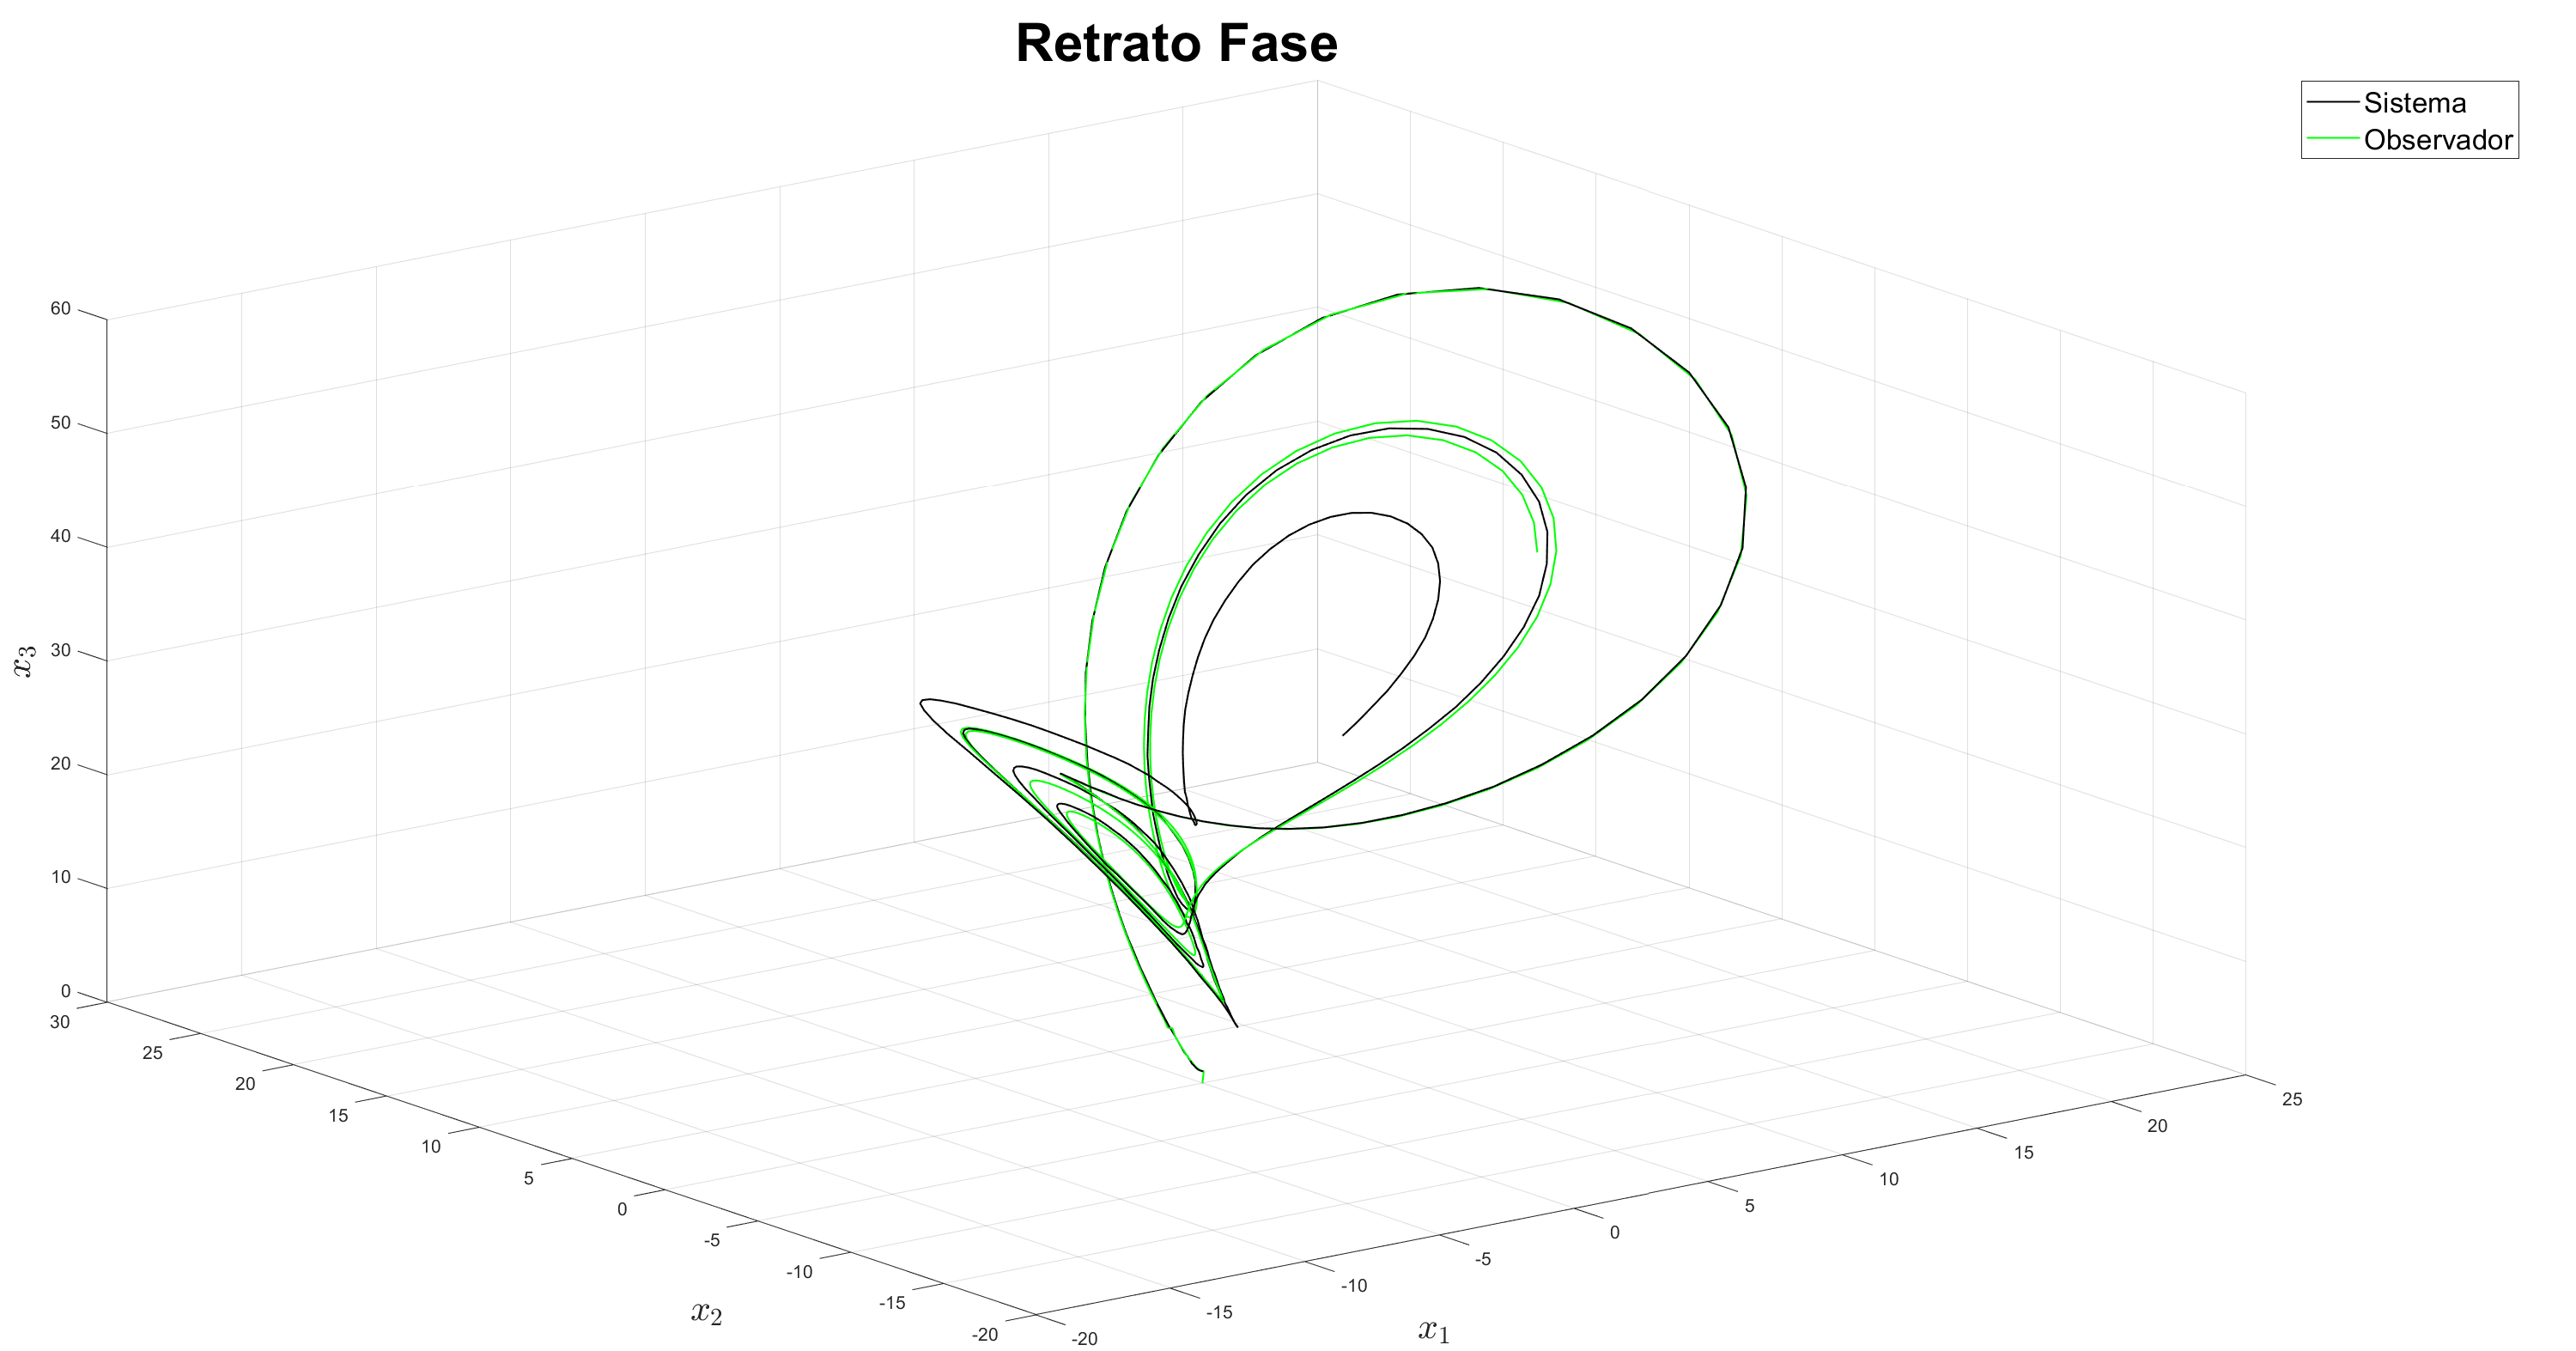
\includegraphics[width=150mm]{img/E1_RetratoFase_Disc.png}
	\caption{Se observa el sistema de Lorenz y su observador}
	\label{img:lorenzD1}
\end{figure}

El sistema de Lorenz se simuló con los siguientes parametros: $\sigma = 10, \ r = 28, \ b = 8/3$.La progresión de los estados en el tiempo se observan en la siguiente figura:

\begin{figure}[H]
	\centering
	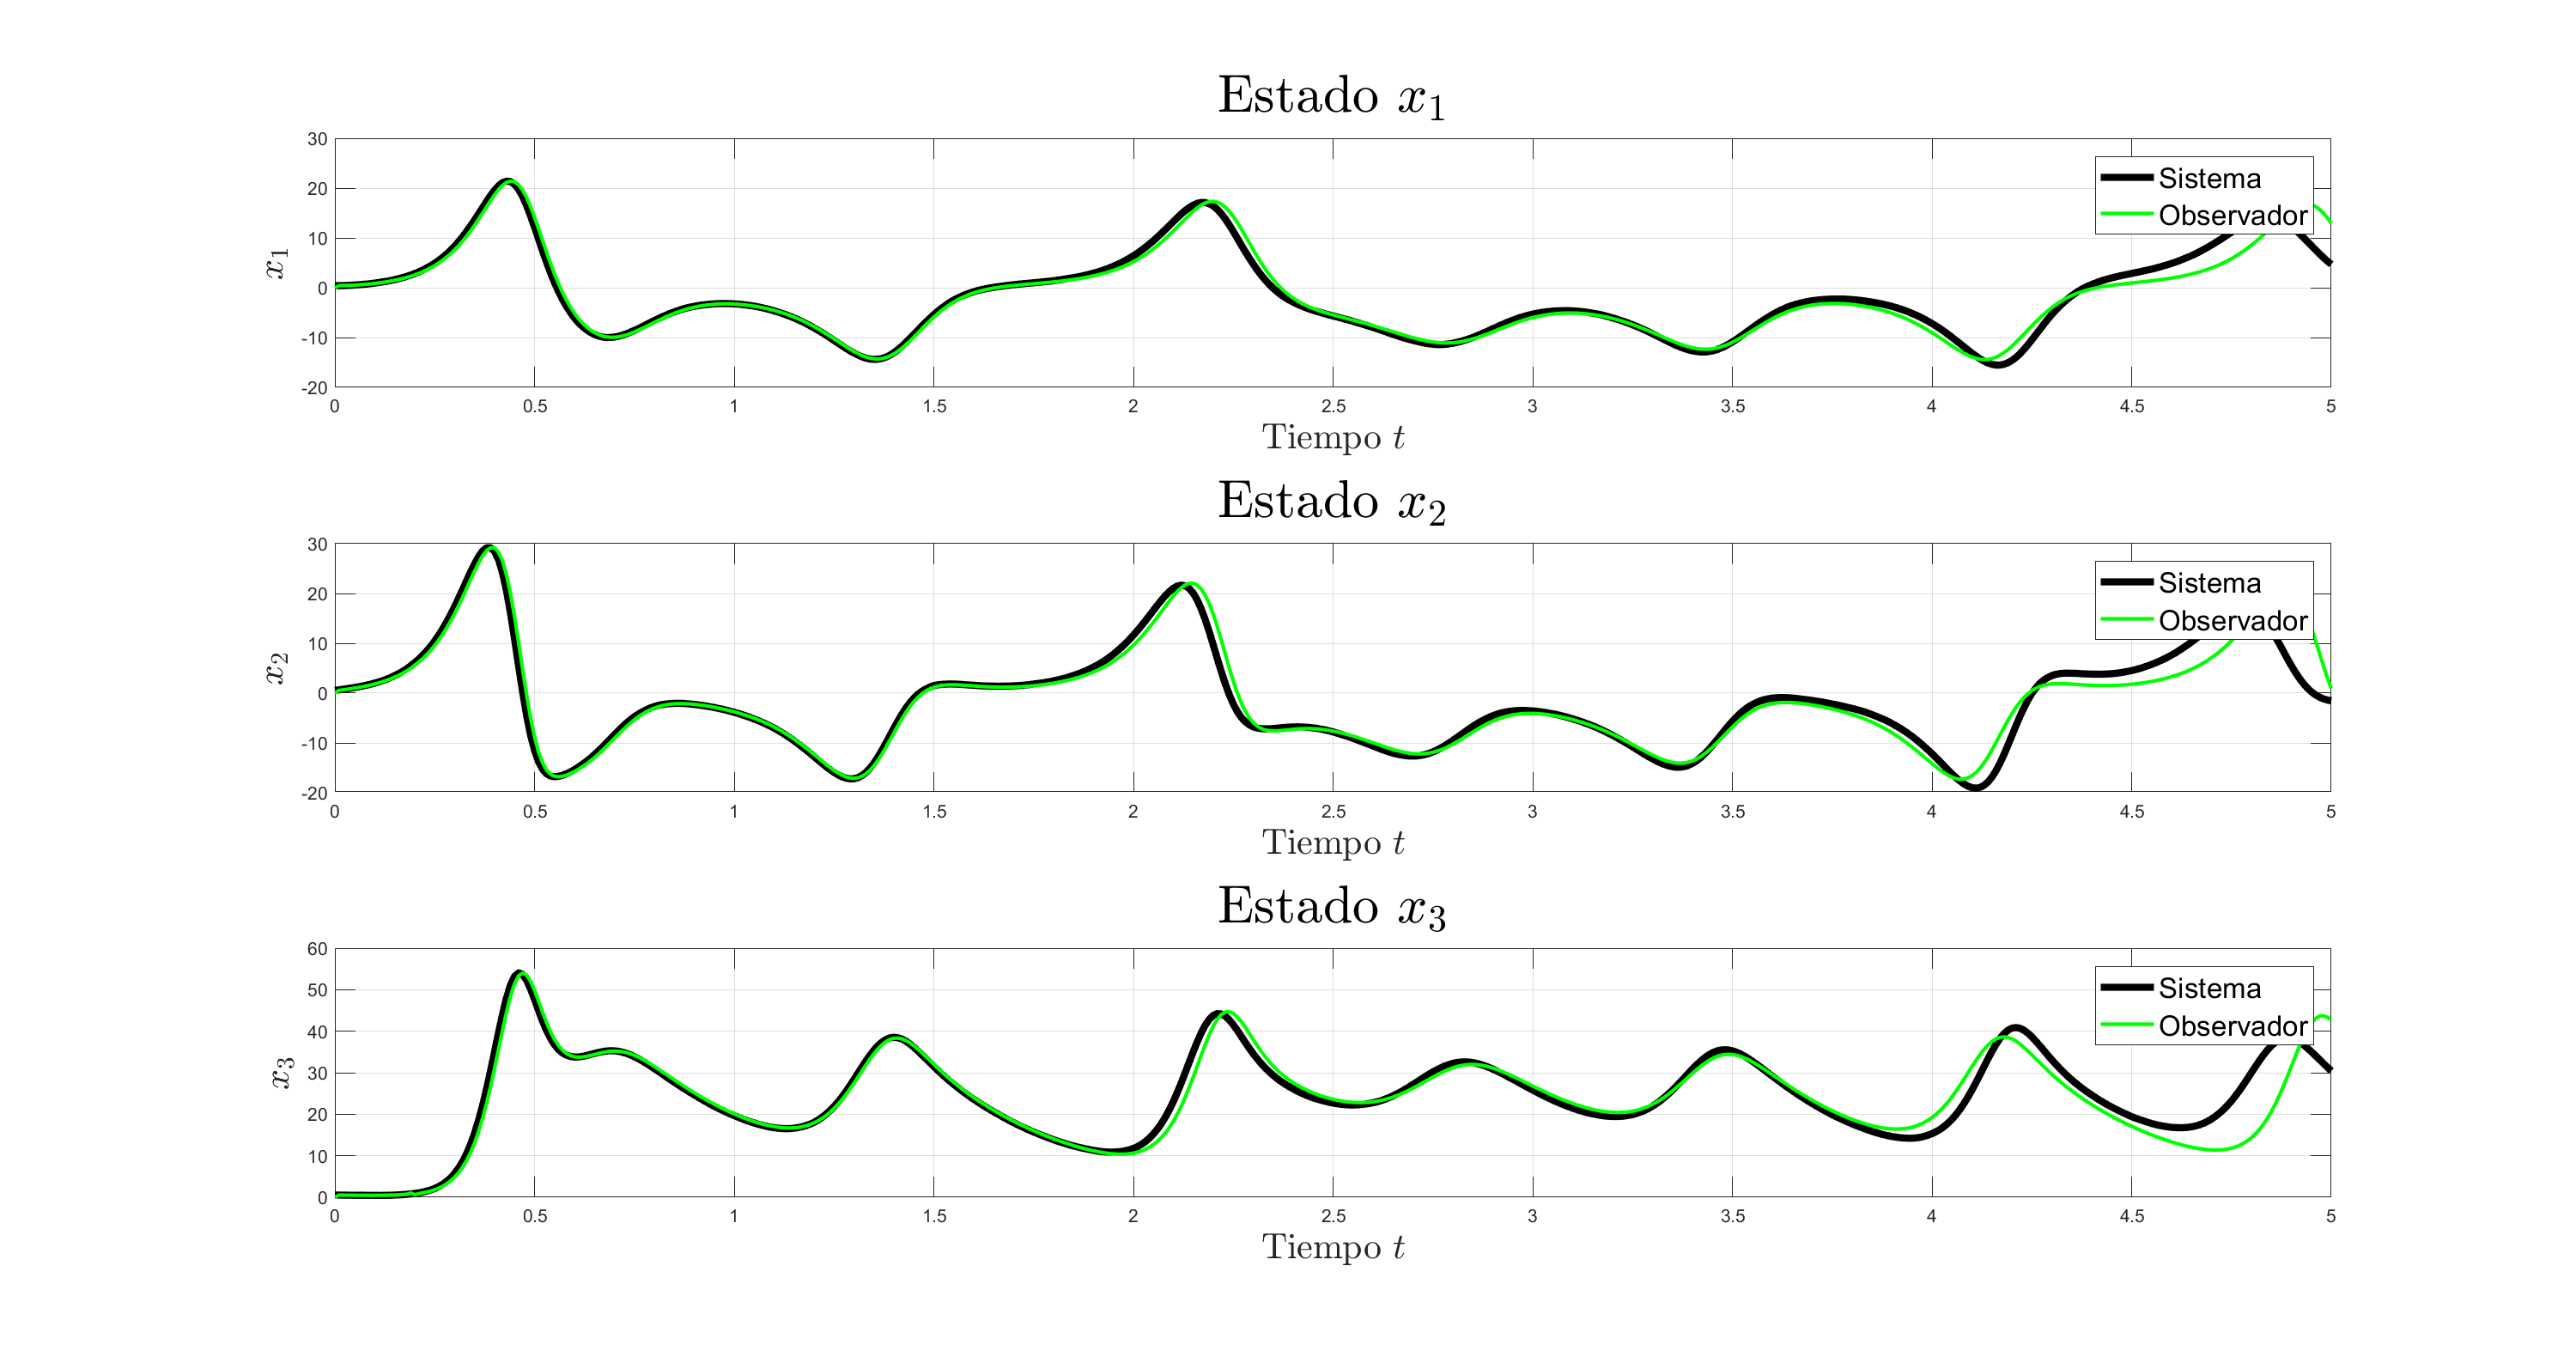
\includegraphics[width=150mm]{img/E1_Estados_Disc.png}
	\caption{Progresión de los estados en el tiempo}
	\label{img:lorenzD2}
\end{figure}

En base a la figura anterior (\ref{img:lorenzD2}), se obtuvieron los errores del sistema original con el observador.

\begin{figure}[H]
	\centering
	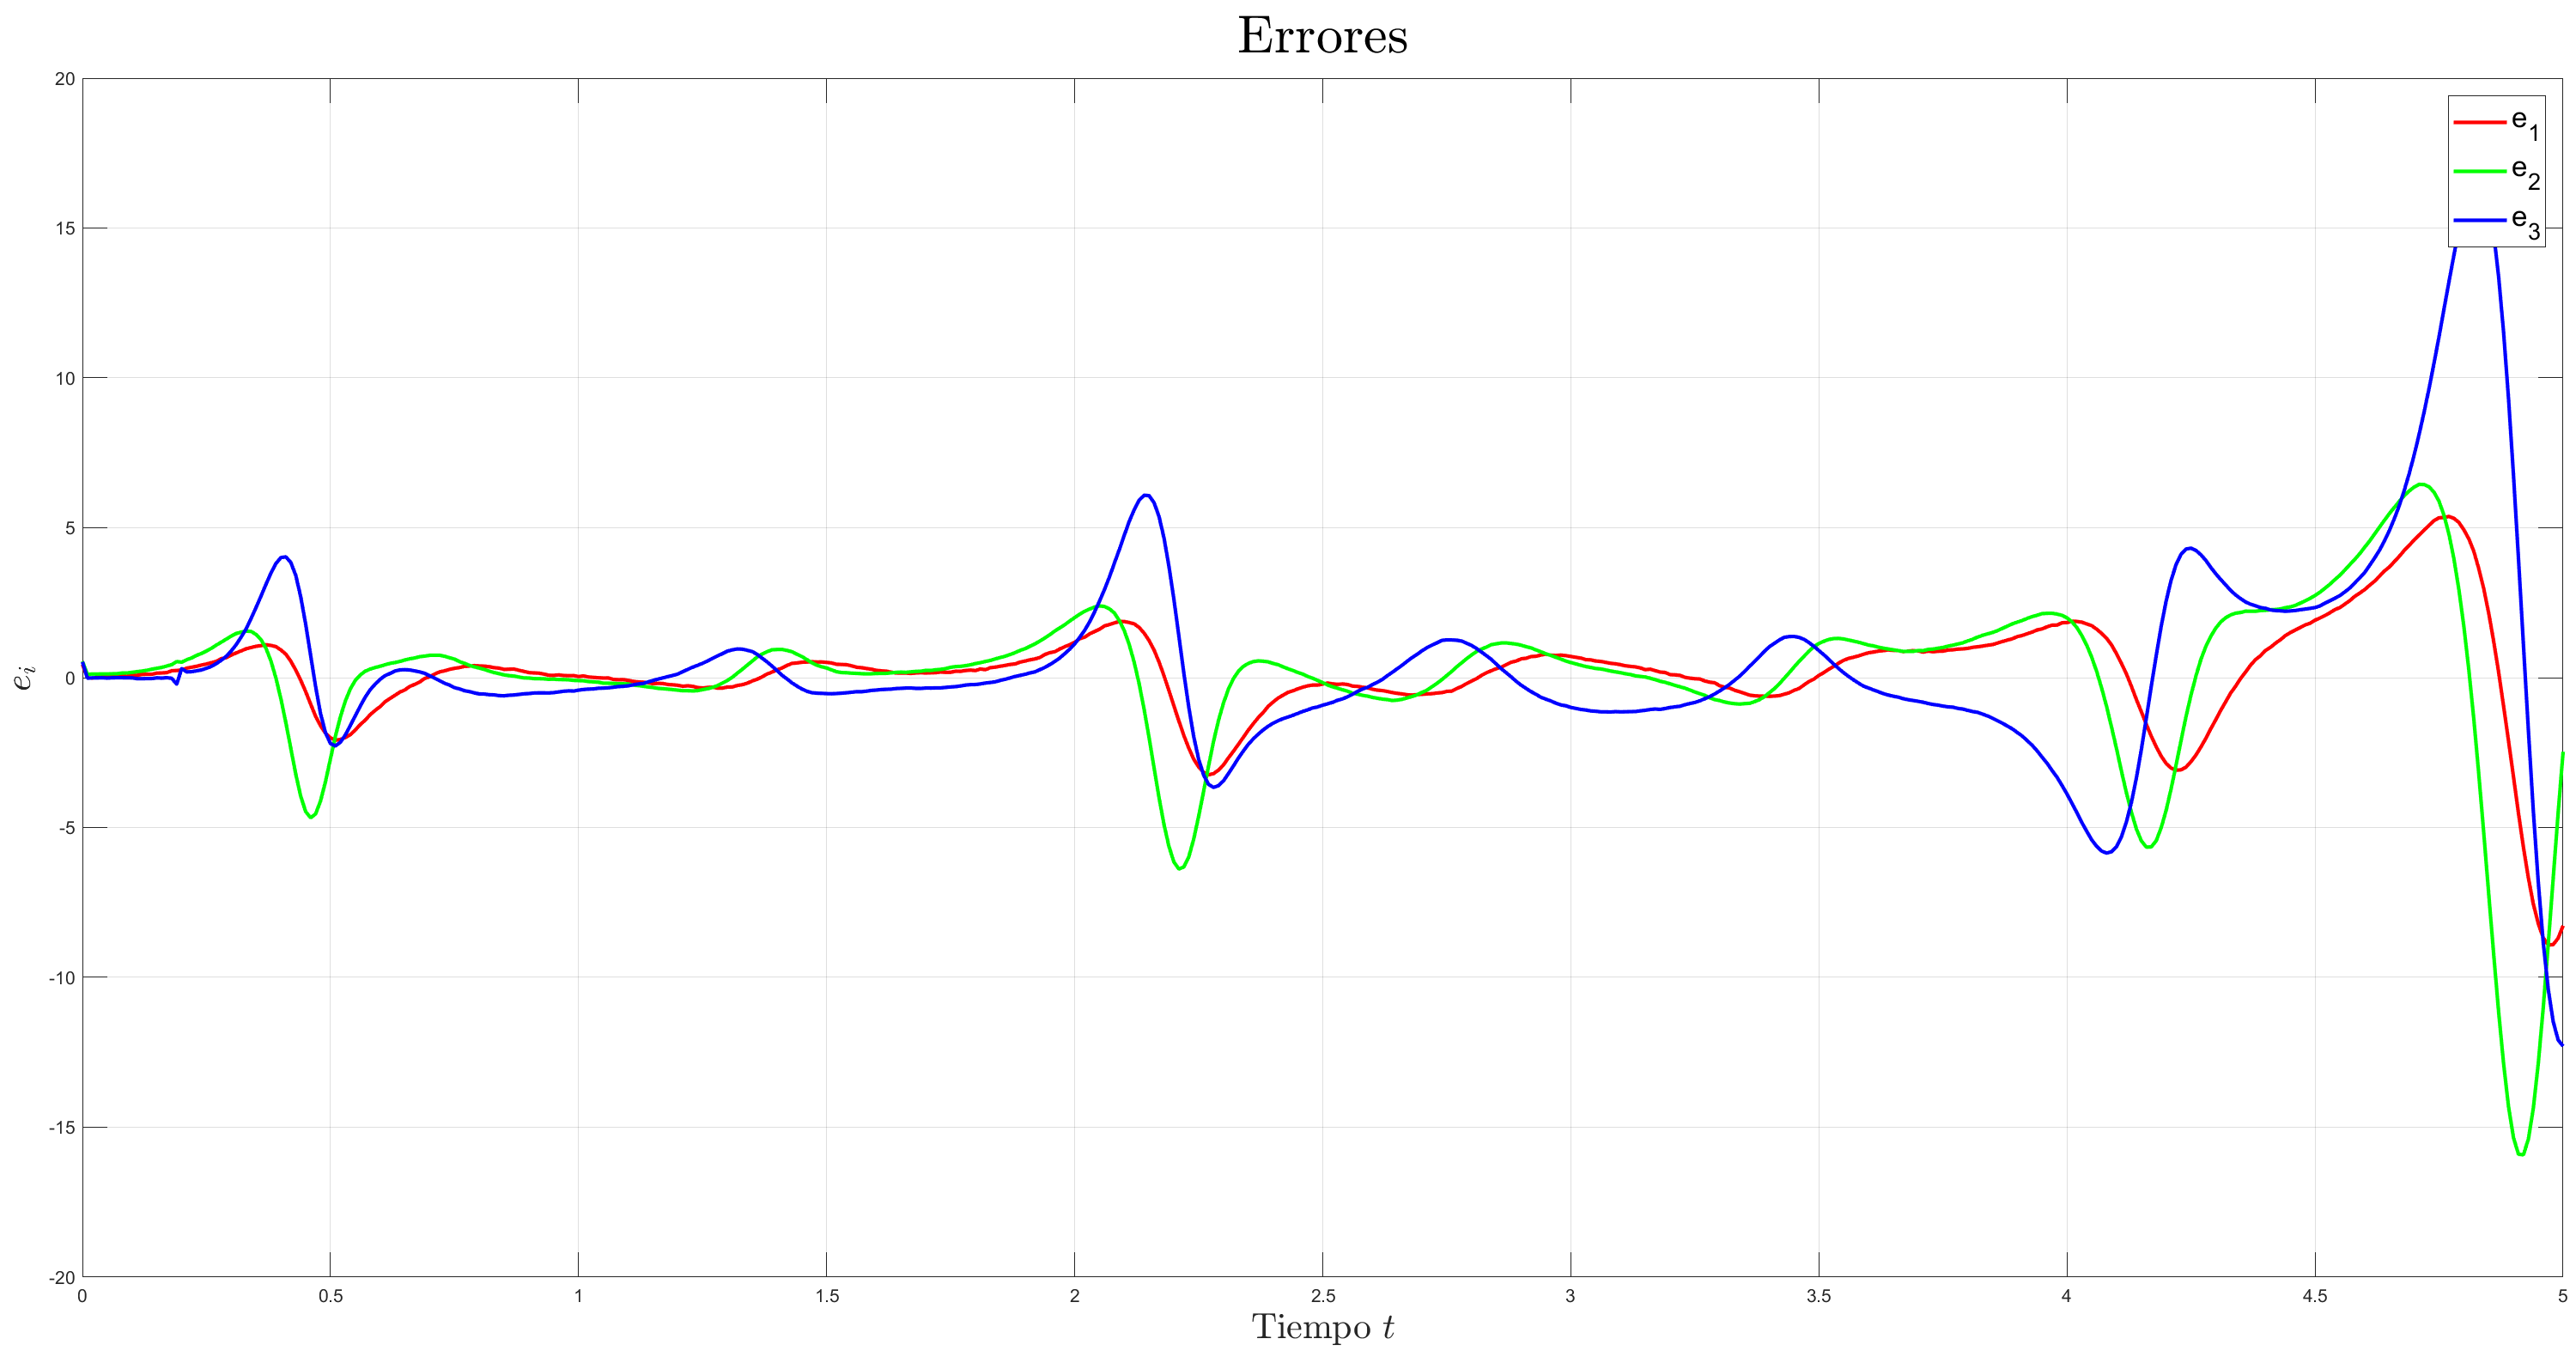
\includegraphics[width=150mm]{img/E1_Errores_Disc.png}
	\caption{Error del sistema de Lorenz y su observador}
	\label{img:lorenzD3}
\end{figure}

Con la simulación de forma continua se obtuvo el siguiente retrato fase:

\begin{figure}[H]
	\centering
	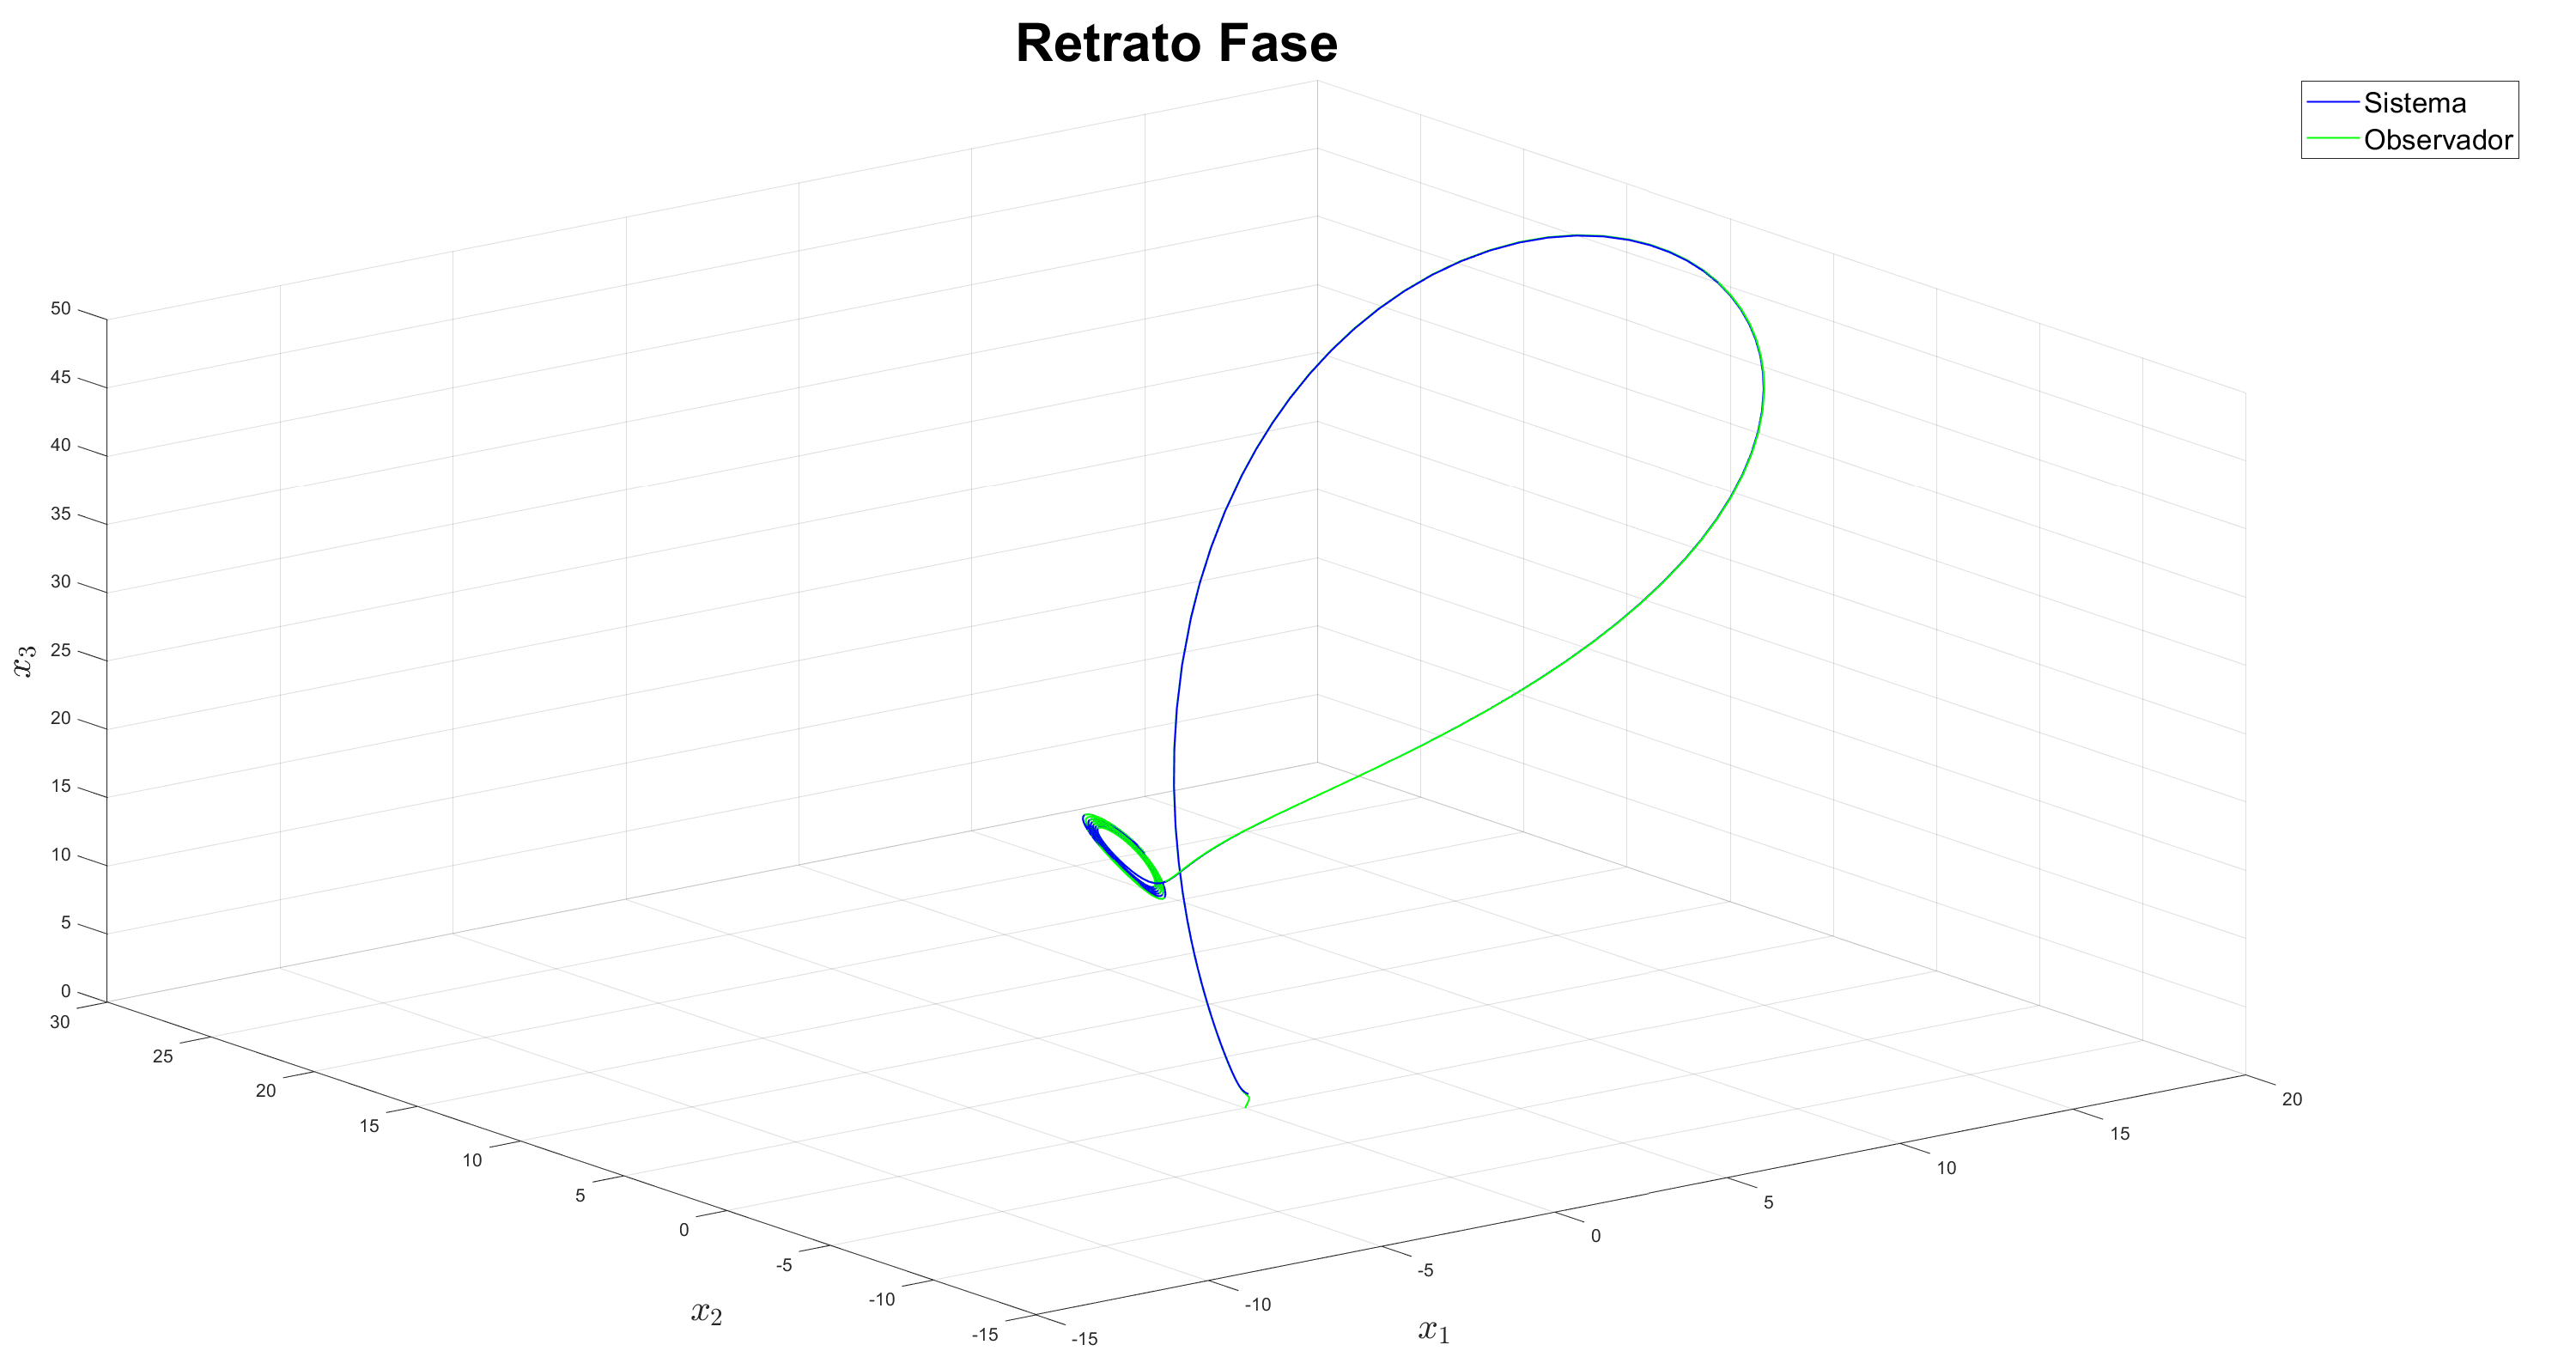
\includegraphics[width=150mm]{img/E1_RetratoFase_Cont.png}
	\caption{Se observa el sistema de Lorenz y su observador}
	\label{img:lorenzD4}
\end{figure}

El sistema fue simulado con los mismos paramteros que la simulación discreta. La progresión de los estados en el tiempo se observan en la siguiente figura:

\begin{figure}[H]
	\centering
	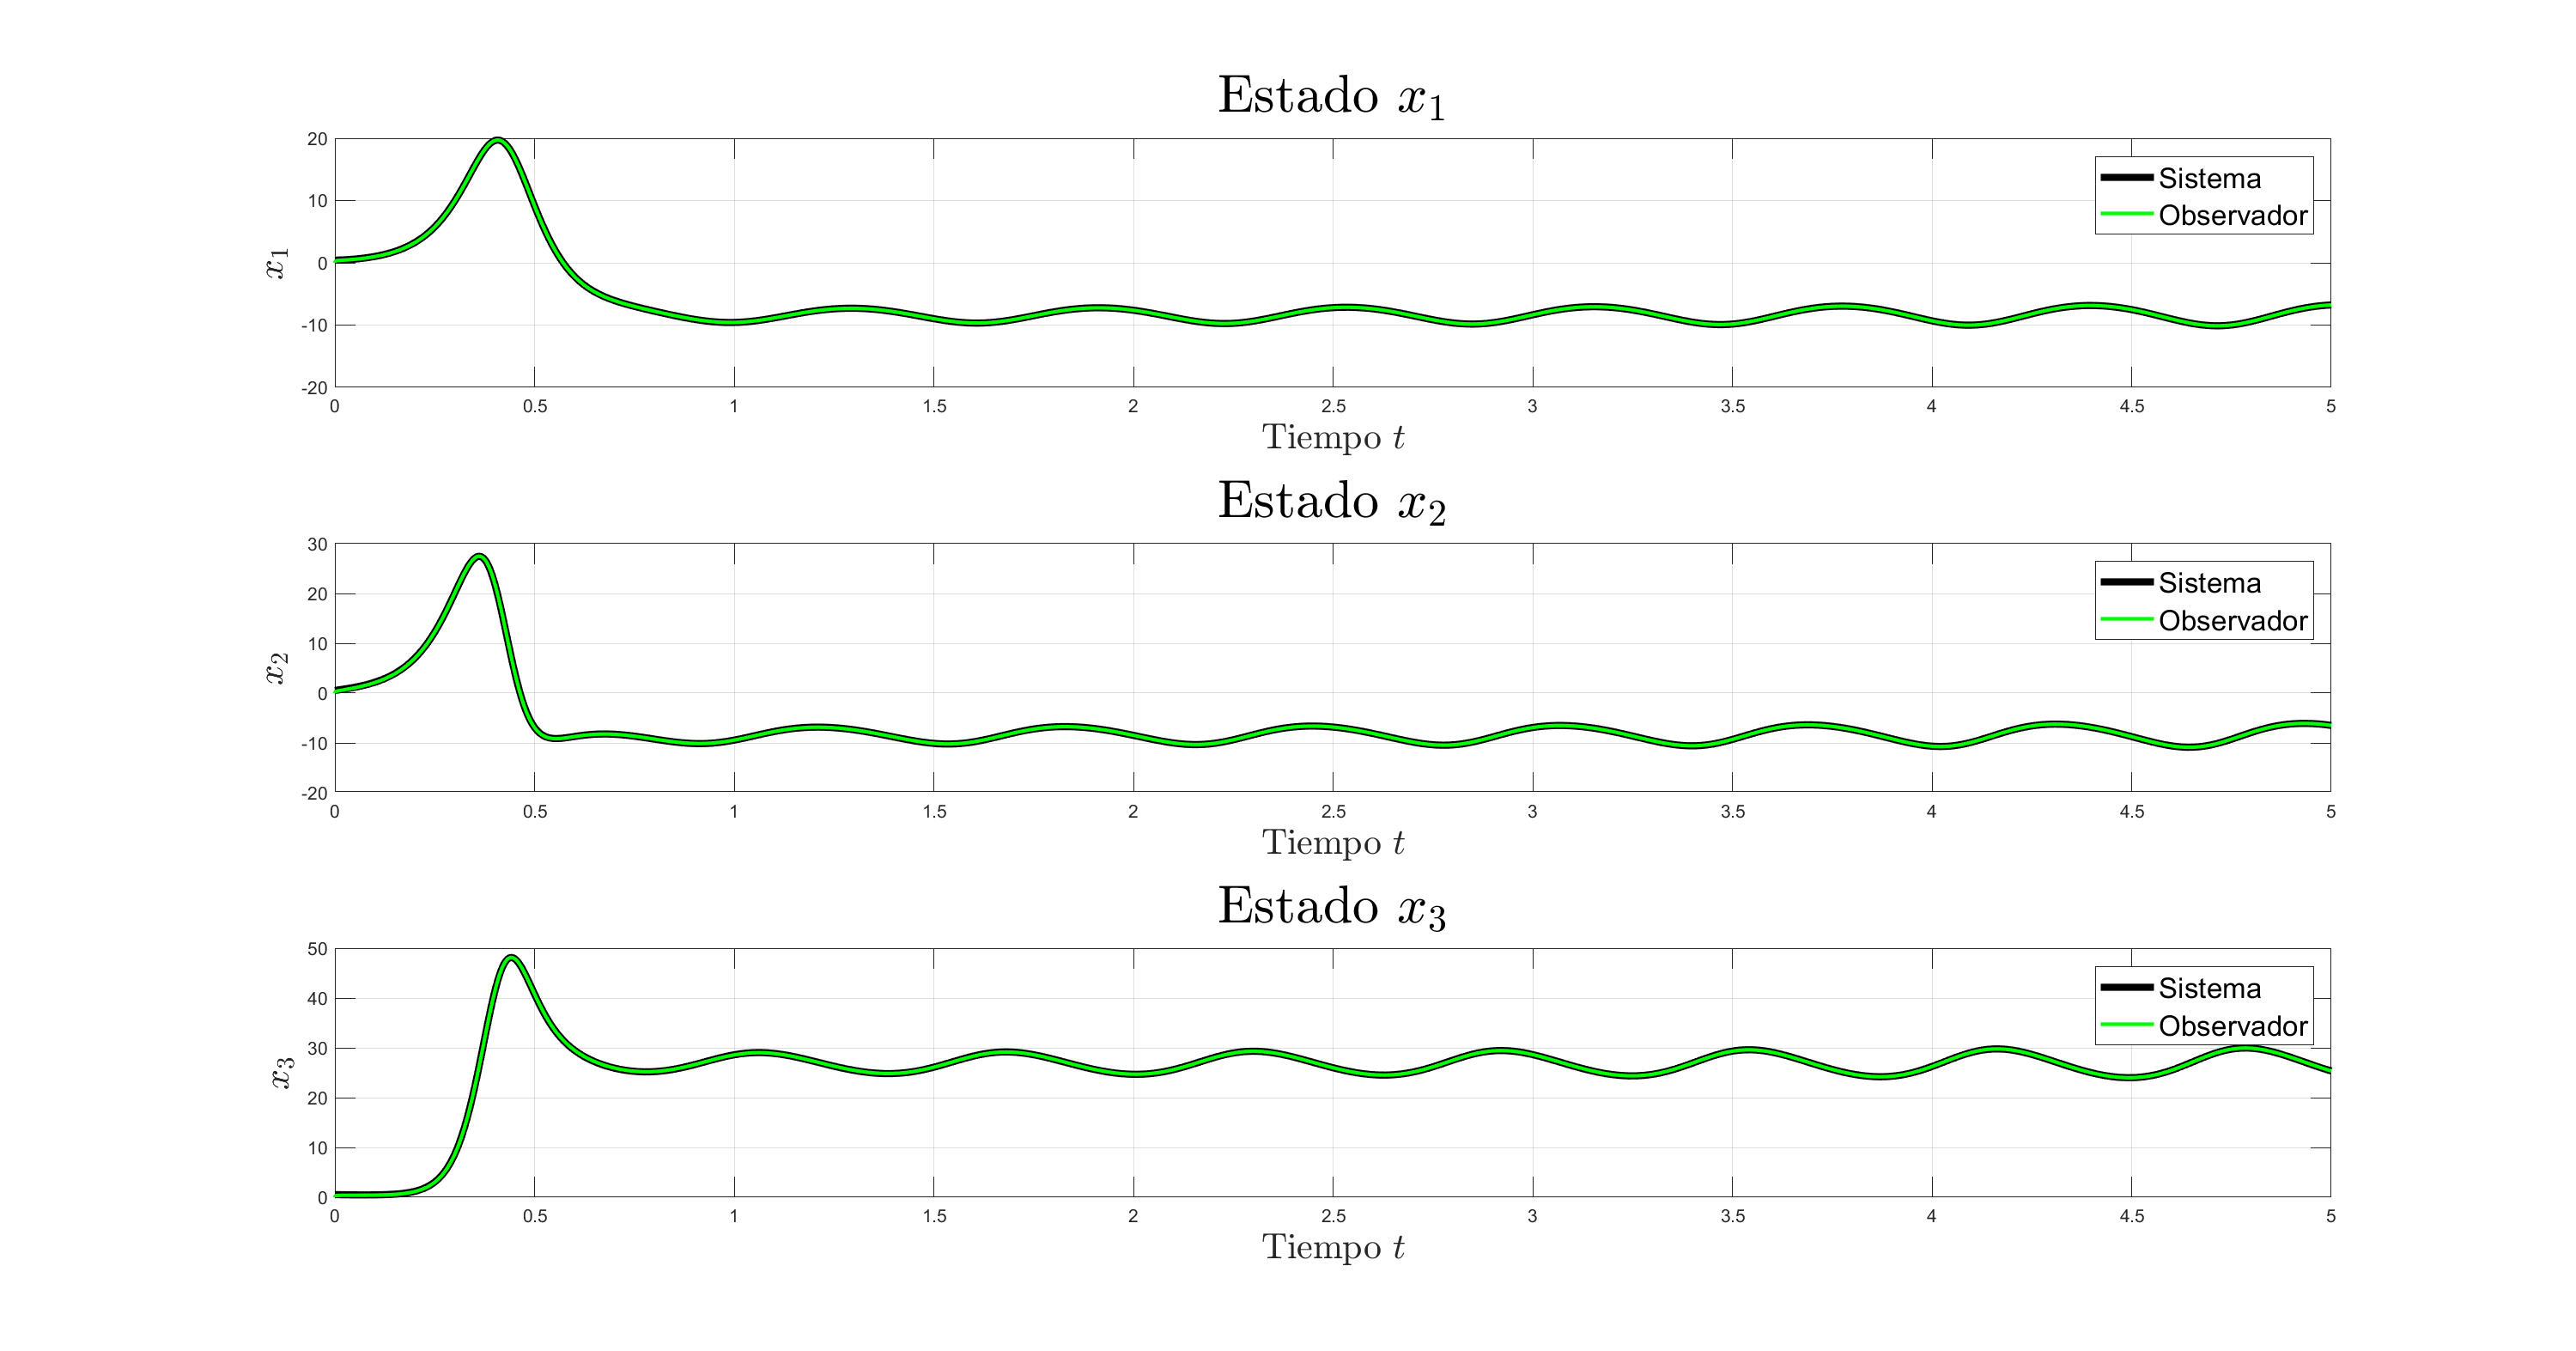
\includegraphics[width=150mm]{img/E1_Estados_Cont.png}
	\caption{Progresión de los estados en el tiempo}
	\label{img:lorenzD5}
\end{figure}

En base a la figura anterior (\ref{img:lorenzD5}), se obtuvieron los errores del sistema original con el observador.

\begin{figure}[H]
	\centering
	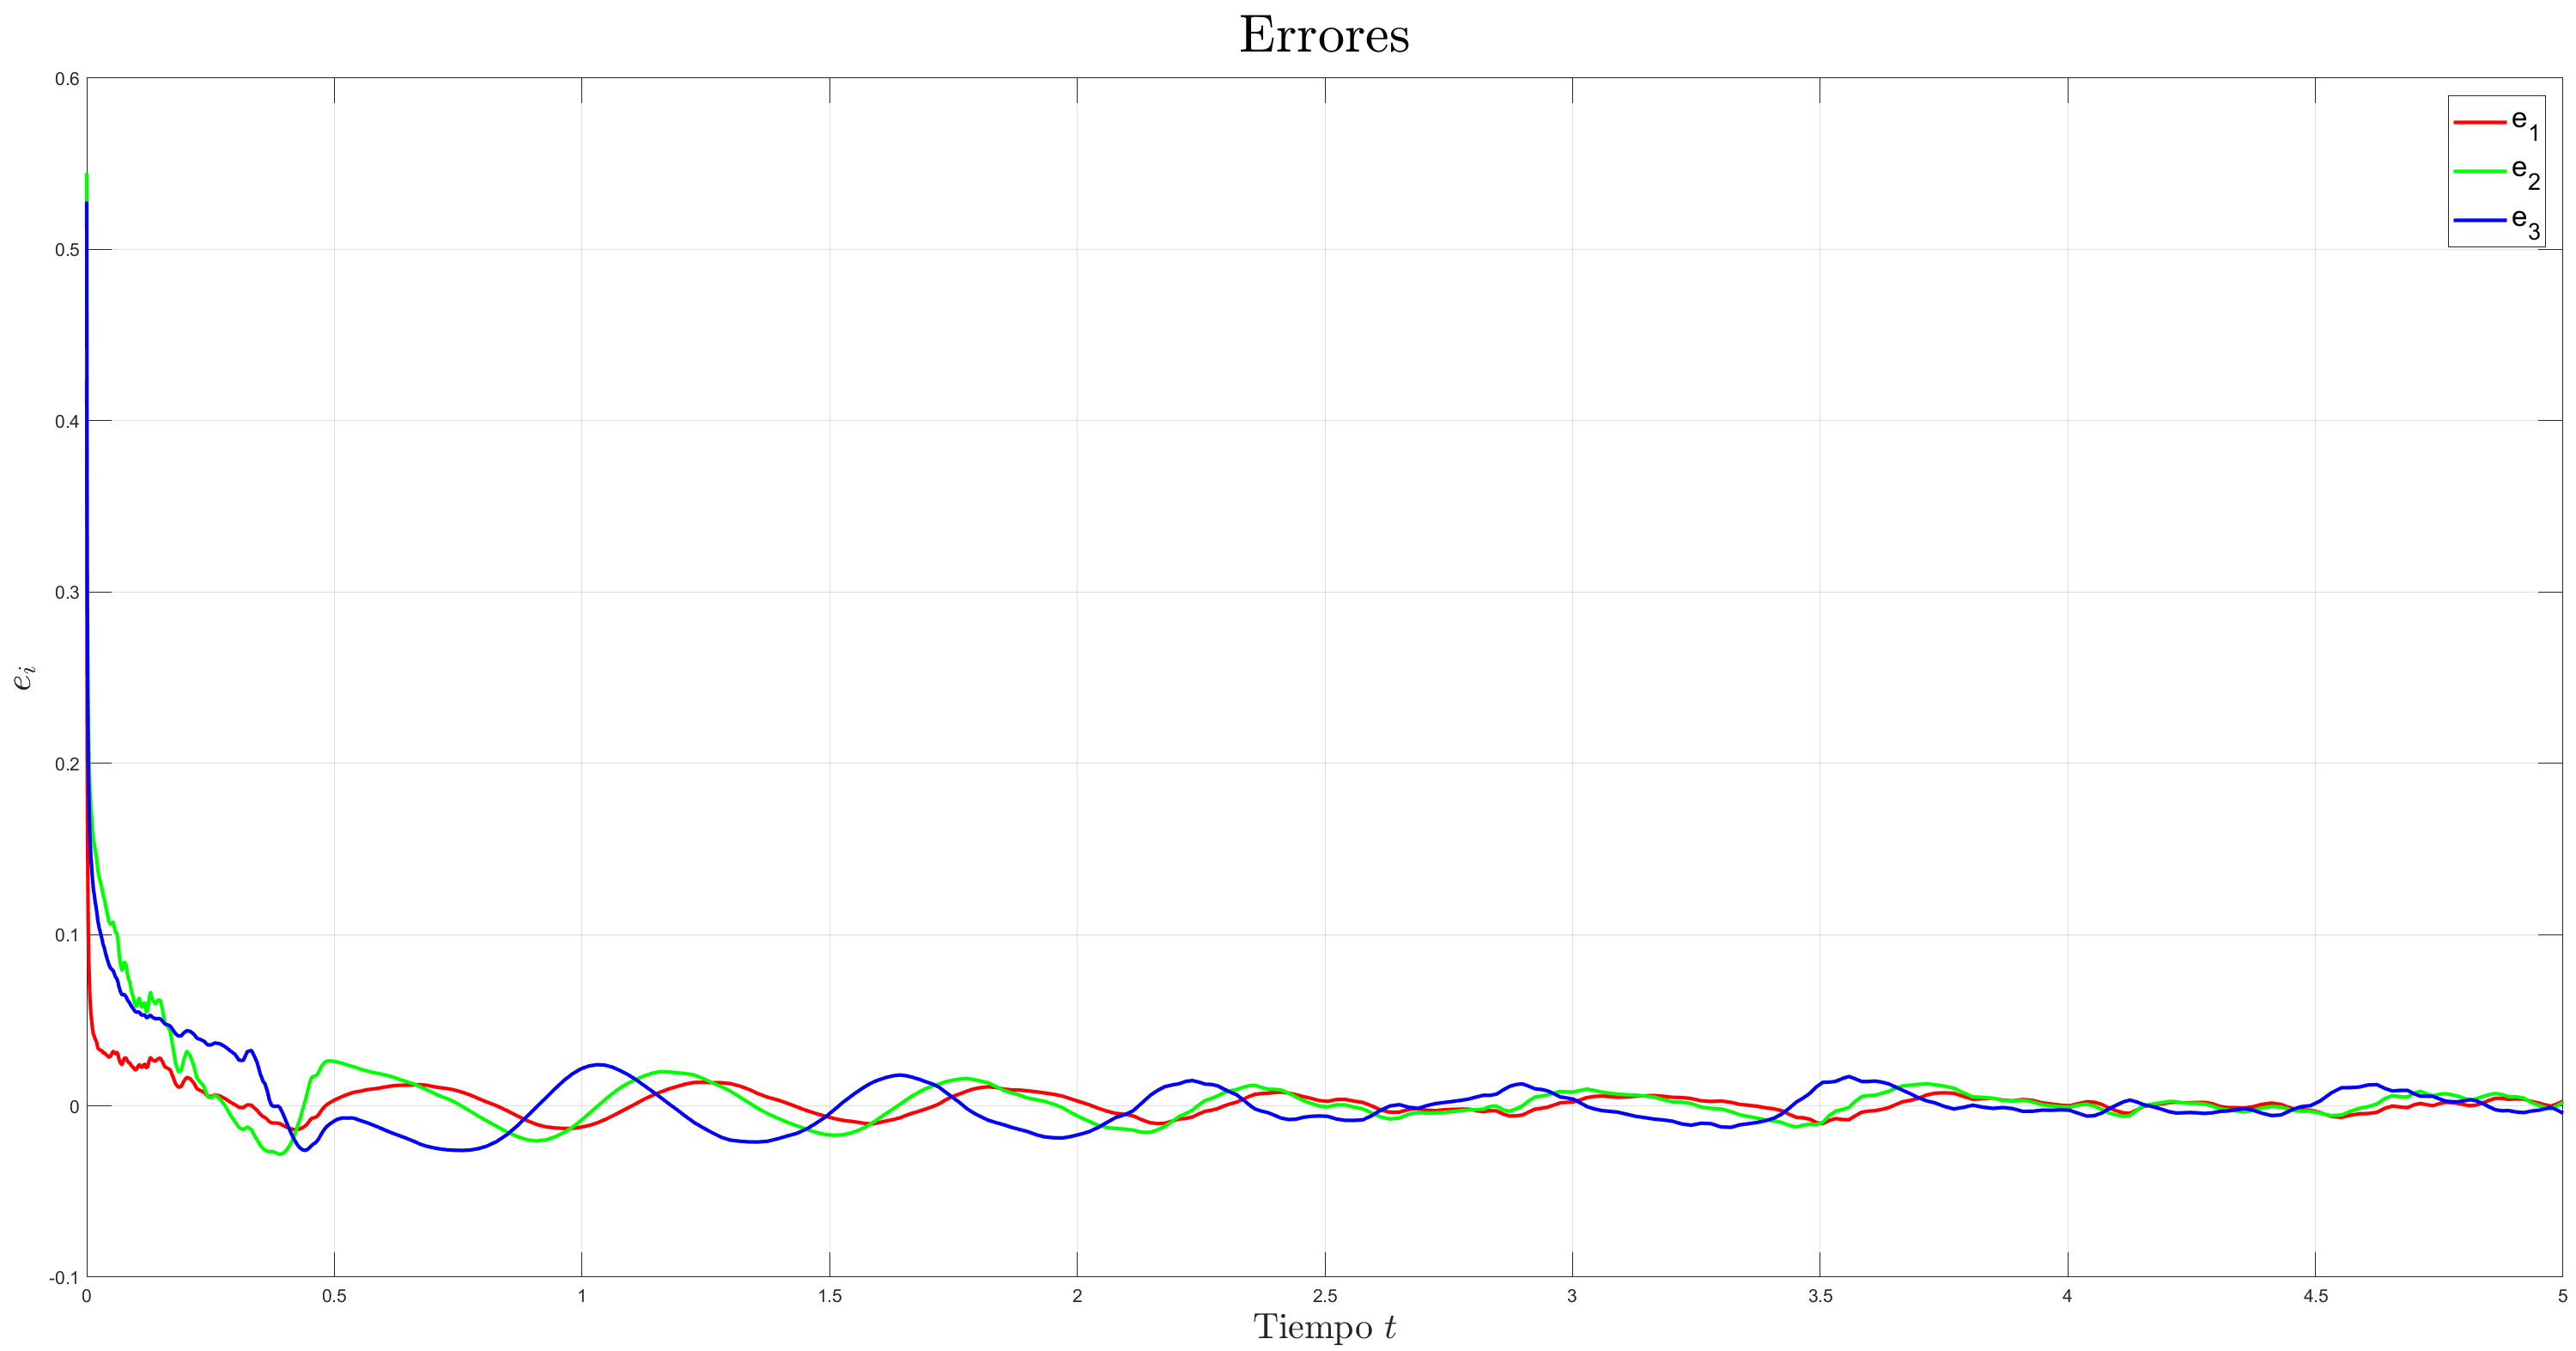
\includegraphics[width=150mm]{img/E1_Errores_Cont.png}
	\caption{Error del sistema de Lorenz y su observador}
	\label{img:lorenzD6}
\end{figure}

\subsection*{Ejercicio 2}

En este ejercicio se utiliza el sistema de Rossler (ecuación \ref{eq:rossler}) al cual se le aplica una señal constante y/o de variacion lenta en el tiempo en el valor de $\lambda$. Esta señal es enviada de manera encriptada dentro del sistema por medio de la salida $y$.

\begin{equation}\label{eq:rossler}
	\begin{array}{c}
		\dot{x}_1 = -x_2 - x_3\\
		\dot{x}_2 = x_1 + \lambda x_2\\
		\dot{x}_3 = 2 + (x_1 - 4)x_3\\
		y = x_3
	\end{array}
\end{equation}

Para recrear la señal $\lambda$ es necesario que se pueda hacer un observador el cual se pueda sincronizar con el sistema. Sin embargo un observador del sistema en \ref{eq:rossler} mostrado en \ref{eq:rosslernosinc} no se sincroniza con el sistema. Por lo tanto se realiza el cambio de coordenada siguiente $\xi_1 = x_1, \ \xi_2 = x_2, \ \xi_3 = \log(x_3) $ y se obtiene el sistema 

\begin{equation}\label{eq:rosslernosinc}
	\begin{array}{c}
		\dot{\hat{x}}_1 = -\hat{x}_2 - \hat{x}_3\\
		\dot{\hat{x}}_2 = \hat{x}_1 + \lambda \hat{x}_2\\
	\end{array}
\end{equation}

\begin{equation}
	\begin{array}{c}
		\dot{x}_1 = -\xi_2 - \xi_3\\
		\dot{x}_2 = \xi_1 + \lambda \xi_2\\
		\dot{x}_3 = \xi_1 + 2e^{-\xi_3} - 4\\
		\bar{y} = \xi_3
	\end{array}
\end{equation}

Con este cambio de coordenadas el observador puede sincronizarse y por lo tanto se puede utilizar en el método de identificación lineal de parametros para reconstruir la señal $\lambda$. Para realizar este proceso se deben de cumplir las siguientes ecuaciones:

\begin{equation}\label{eq:idlinpar}
	\begin{array}{c}
		\dot{w}_i = Kw_i + Lu_i\\
		\hat{y} = \phi_0(w) + \hat{\lambda}\phi_1(w)\\
		\dot{\hat{\lambda}} = -v\phi_1(w)P(\hat{y} - \bar{y})\\
		\dot{P} = -v( \phi_1(w)^2P^2 - \gamma P )
	\end{array}
\end{equation}

Y utilizando el sistema de Rossler en las ecuaciones de \ref{eq:idlinpar} el cual utiliza un estimador de mínimos cuadrados con factor de olvido se obtienen las siguientes ecuaciones diferenciales a resolver.

\begin{equation}
	\begin{array}{l}
		\dot{w}_{01} = w_{02}\\
		\dot{w}_{02} = w_{03}\\
		\dot{w}_{03} = -k_0w_{01} - k_1w_{02} - k_2w_{03} + \bar{y}\\
		\dot{w}_{11} = w_{12}\\
		\dot{w}_{12} = w_{13}\\
		\dot{w}_{13} = -k_0w_{11} - k_1w_{12} - k_2w_{13} + u_1\\
		\dot{w}_{21} = w_{22}\\
		\dot{w}_{22} = w_{23}\\
		\dot{w}_{23} = -k_0w_{21} - k_1w_{22} - k_2w_{23} + u_2\\
		\dot{\hat{\lambda}} = -v\phi_1(w)P(\hat{y} - \bar{y})\\
		\dot{P} = -v( \phi_1(w)^2P^2 - \gamma P )
	\end{array}
\end{equation}

En donde se define $\phi_0(w) = k_0w_{01} + (k_1 - 1)w_{02} + k_2w_{03} + w_{12} + w_{21} + w_{23}$, $\phi_1(w) = w_{03} - w_{11} - w_{22}$ y $u_0 = \xi_3$, $u_1 = -x_3$, $u_2 = (2/x_3) - 4$. Y el resulatdo de la integracion de $\hat{\lambda}$ es la aproximación a la señal de $\lambda$.\\

\subsubsection*{Resultados}

En la figura \ref{img:rossler1} se observa el retrato fase del sistema. Donde se observa el movimiento caótico del sistema y en la figura \ref{img:rossler2} se observa la progresión de los estados en el tiempo y hay que notar que la señal enviada del sistema es el tercer estado con la cual se va a aproximar el valor de $\lambda$. 

\begin{figure}[H]
	\centering
	\includegraphics[width=150mm]{img/E2_RetratoFase.png}
	\caption{Retrato Fase del sistema de Rossler}
	\label{img:rossler1}
\end{figure}

\begin{figure}[H]
	\centering
	\includegraphics[width=150mm]{img/E2_Estados.png}
	\caption{Progresión de los estados en el tiempo}
	\label{img:rossler2}
\end{figure}

En la figura \ref{img:rossler3} se observa como la señal recuperada $\hat{\lambda}$ se acerca a la señal $\lambda$ original. Cuando la señal es constante la señal se recupera en poco tiempo (aproximadamente 5s) y la señal con cambios lentos mantiene un cierto nivel de error,se puede observar en la figure \ref{img:rossler4}, pero mantiene la forma general de la señal $\lambda$.

\begin{figure}[H]
	\centering
	\includegraphics[width=150mm]{img/E2_Lambda.png}
	\caption{$\lambda$ y $\hat{\lambda}$ en el tiempo}
	\label{img:rossler3}
\end{figure}

\begin{figure}[H]
	\centering
	\includegraphics[width=150mm]{img/E2_ErrorLambda.png}
	\caption{Error de $\lambda$}
	\label{img:rossler4}
\end{figure}

\subsection*{Ejercicio 3}


\subsubsection*{Resultados}
\begin{figure}[H]
	\centering
	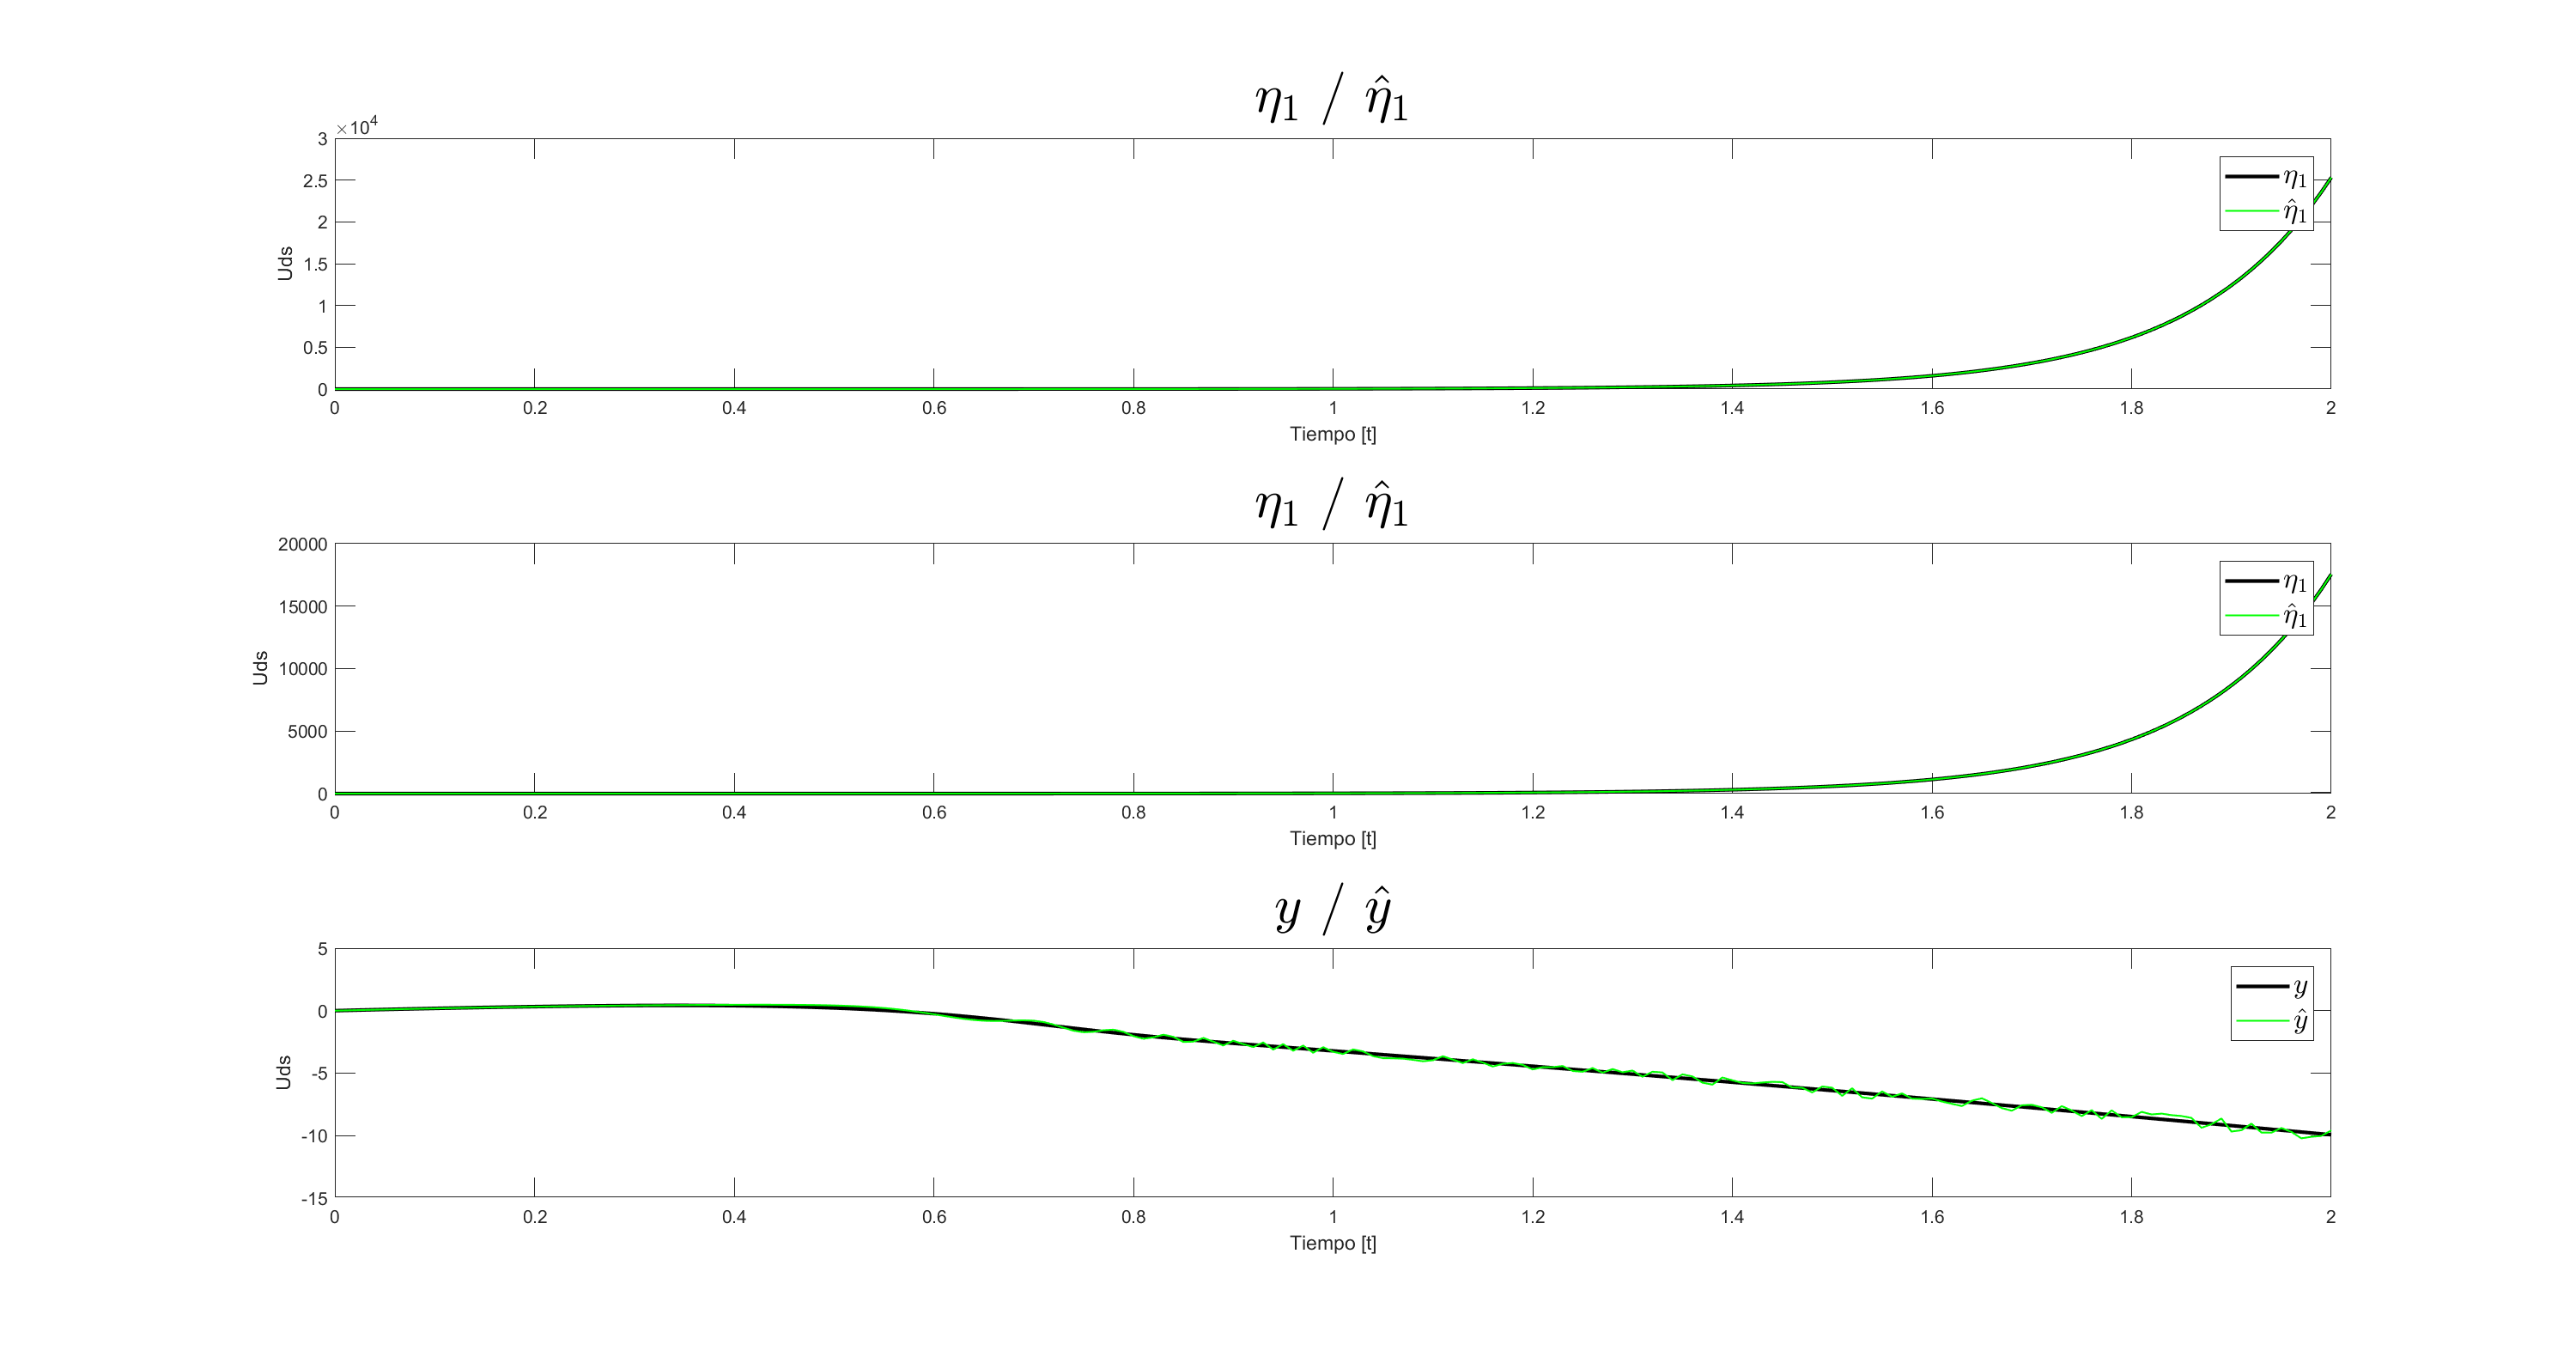
\includegraphics[width=150mm]{img/E3_Estados.png}
	\caption{Progresión de los estados en el tiempo}
	\label{img:rossler5}
\end{figure}

\begin{figure}[H]
	\centering
	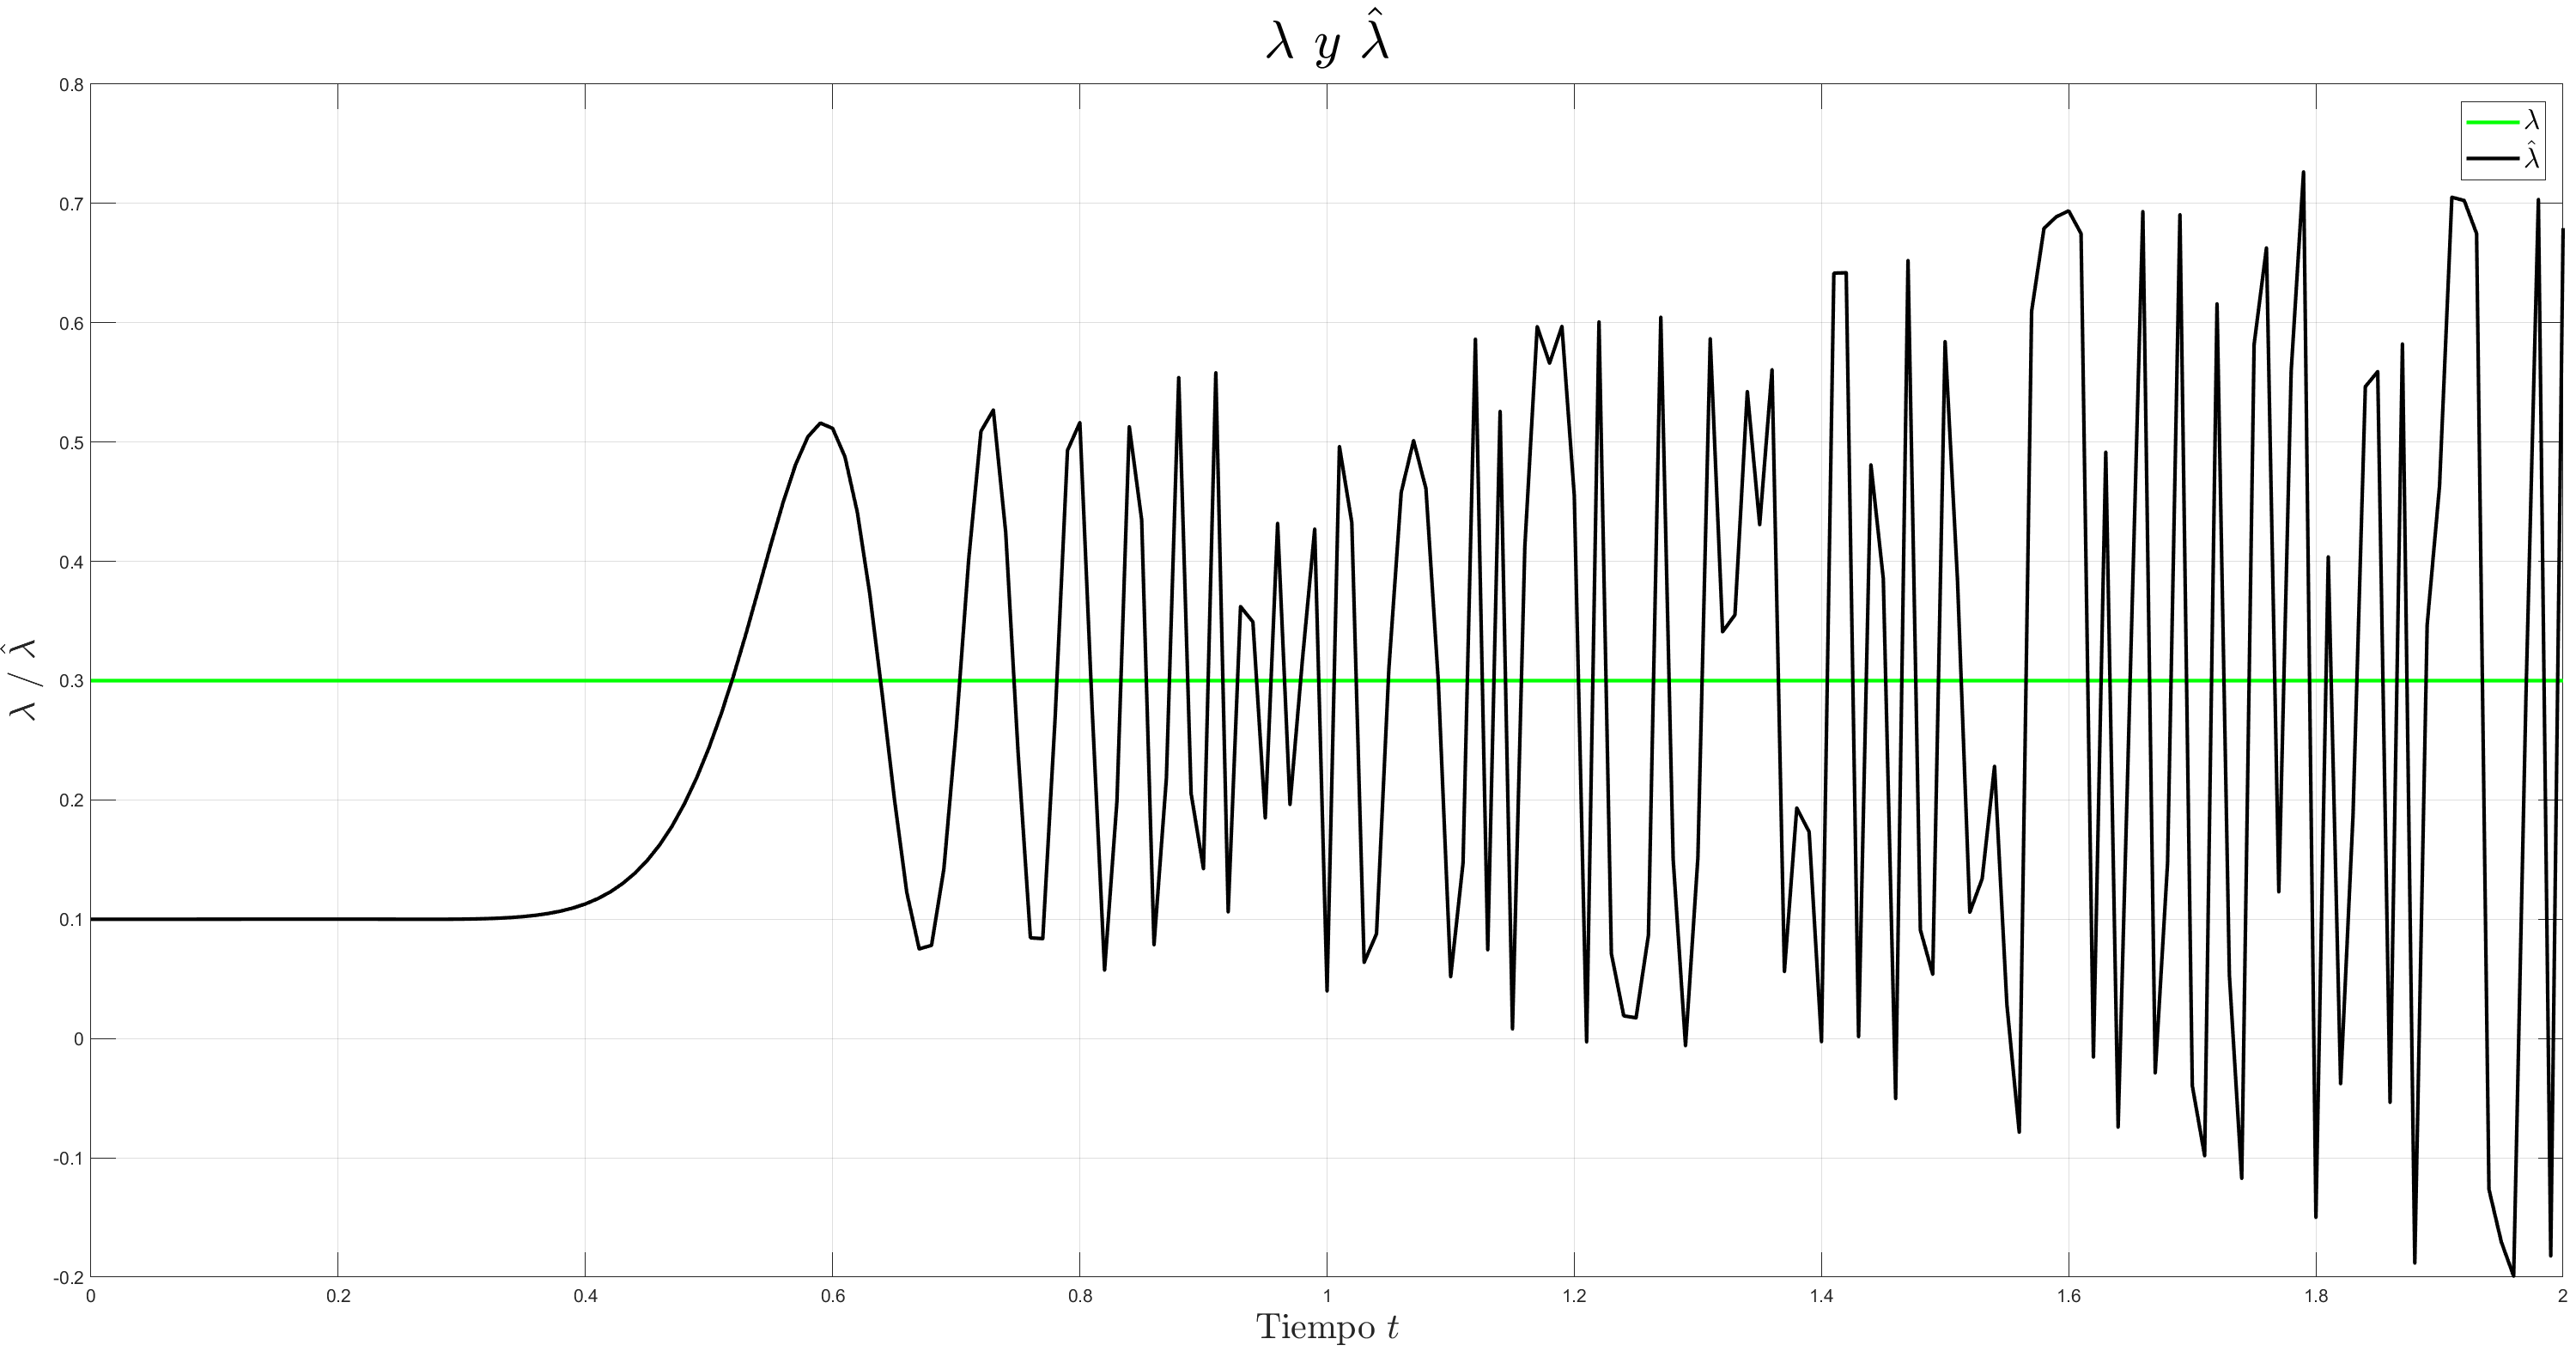
\includegraphics[width=150mm]{img/E3_Lambda.png}
	\caption{$\lambda$ y $\hat{\lambda}$ en el tiempo}
	\label{img:rossler6}
\end{figure}

\begin{figure}[H]
	\centering
	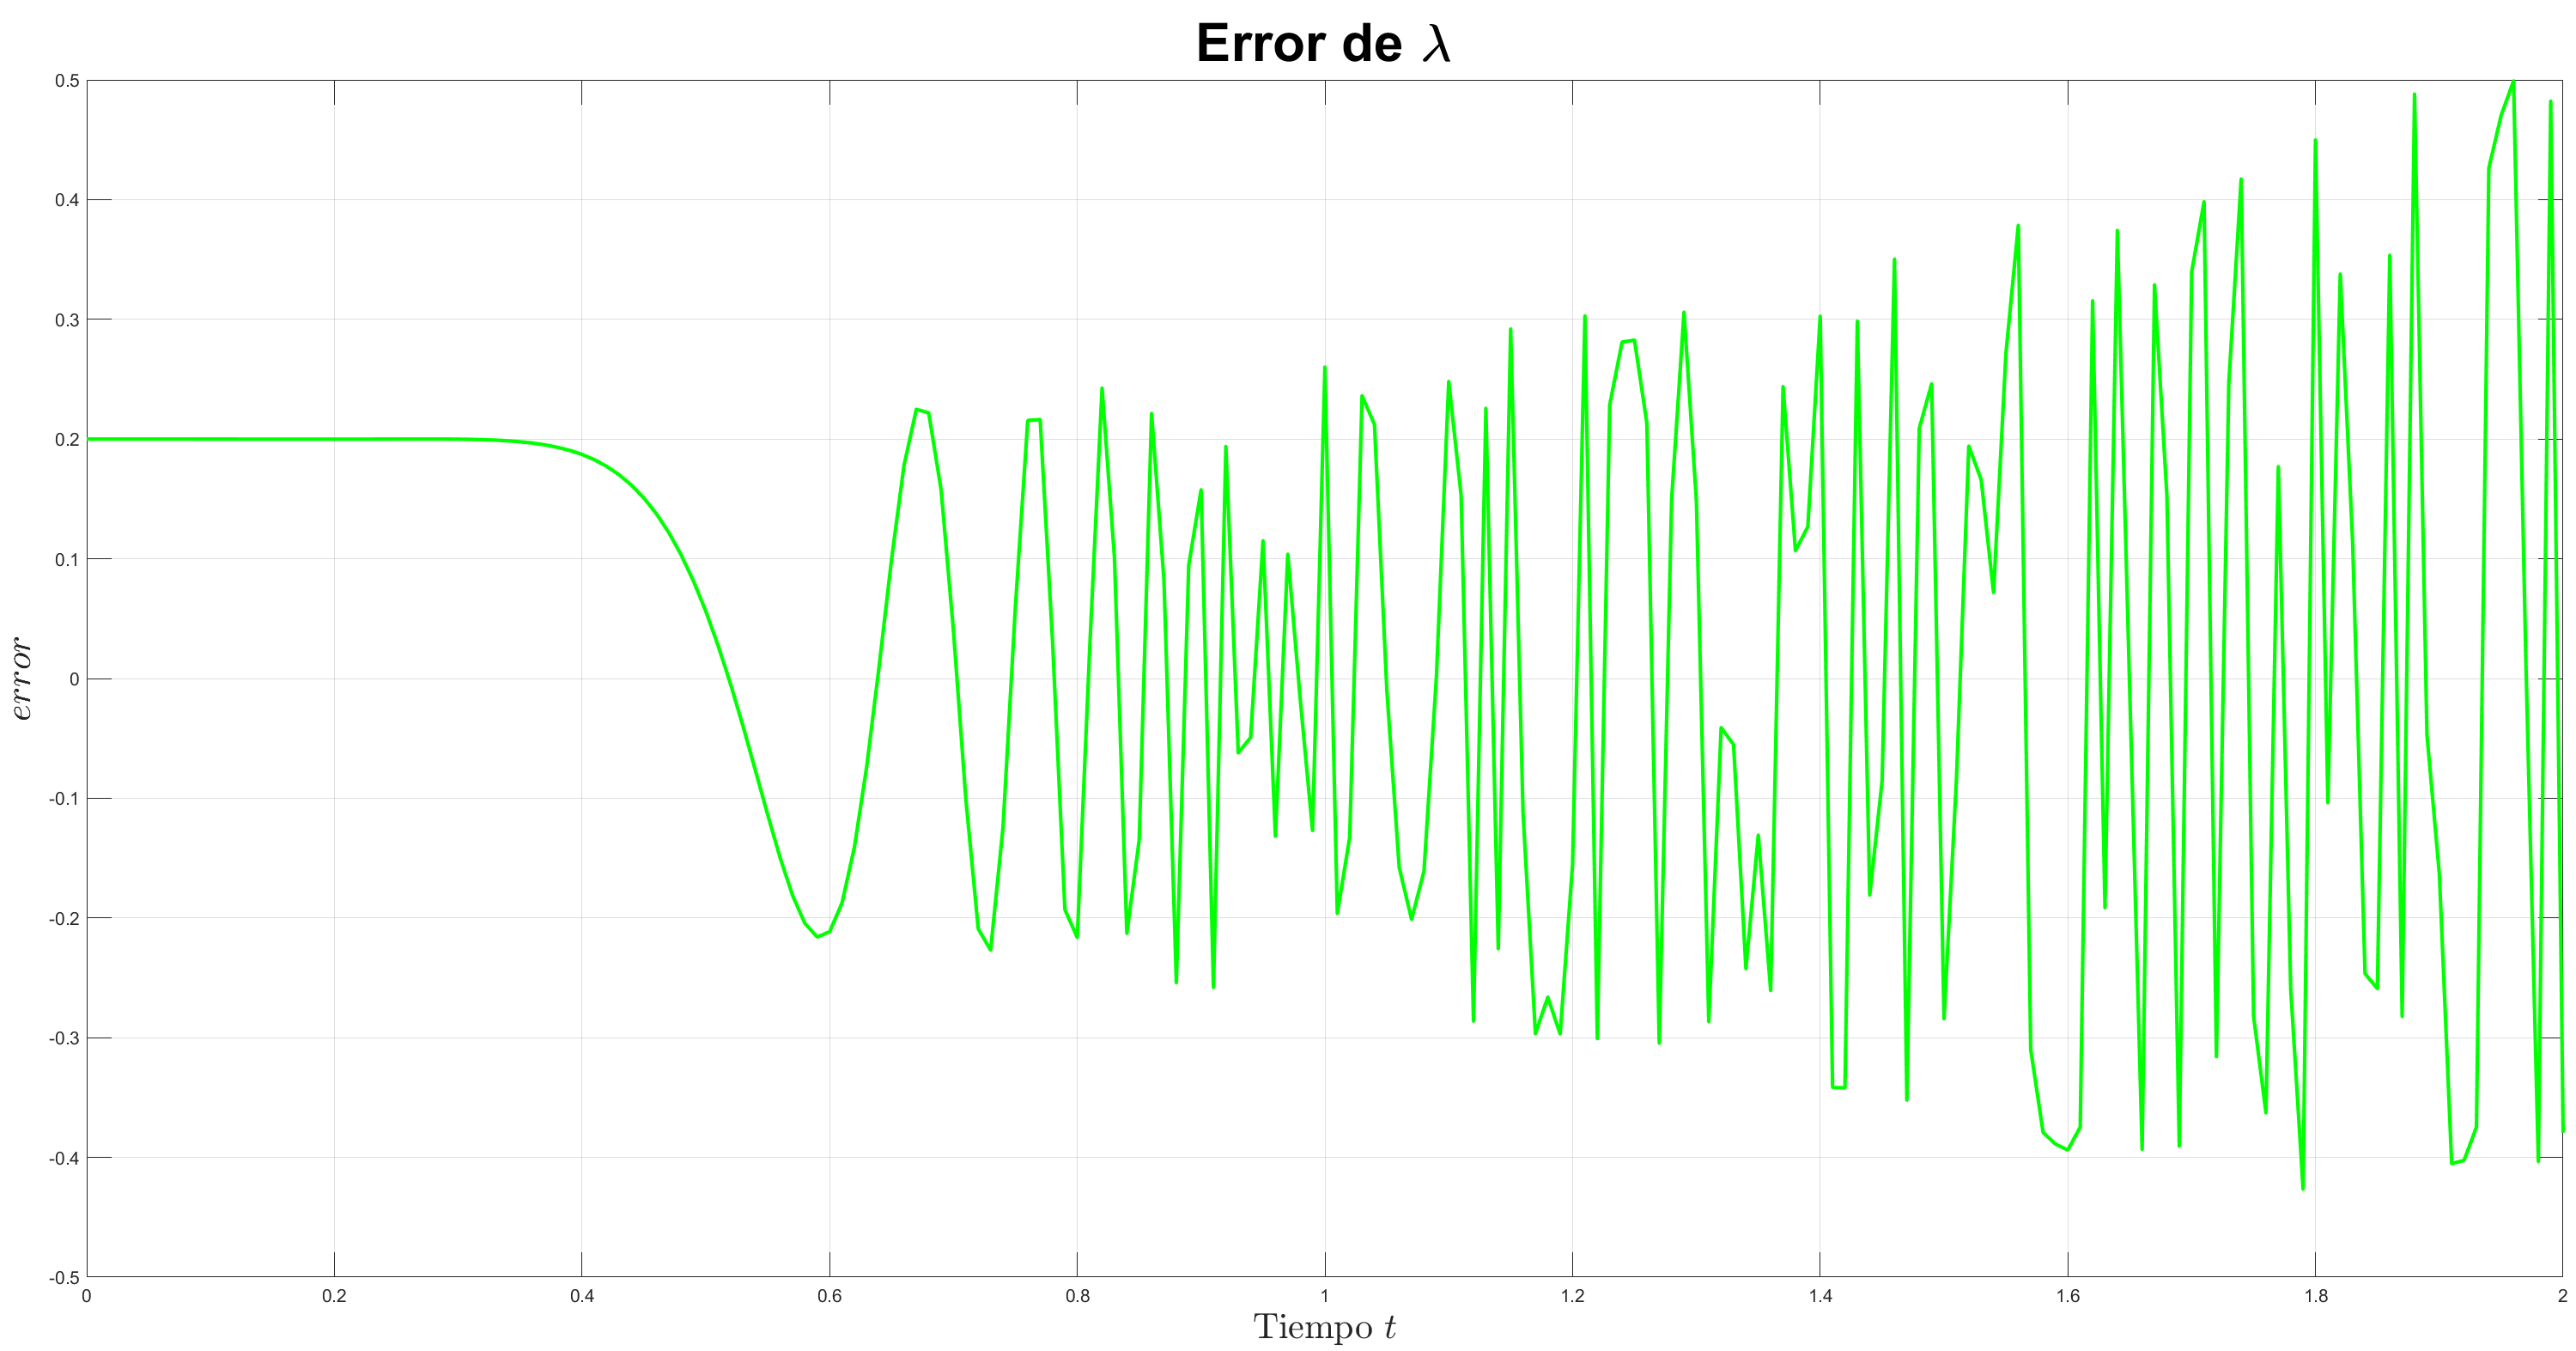
\includegraphics[width=150mm]{img/E3_ErrorLambda.png}
	\caption{Error de $\lambda$}
	\label{img:rossler7}
\end{figure}